\section{Introduction}
\begin{frame}
  \frametitle{Monoliths (really big projects!)}
  \begin{center}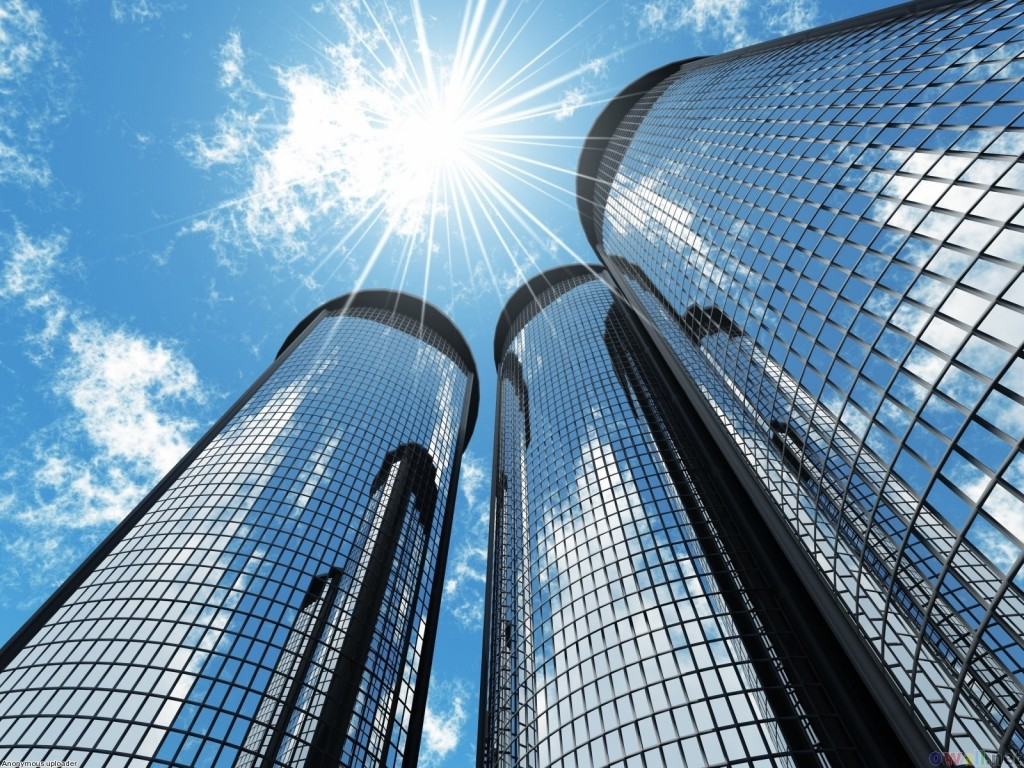
\includegraphics[width=280px]{images/monoliths.jpg}\end{center}
\end{frame}

\begin{frame}
  \frametitle{Monoliths (continued)}
  In terms of \textbf{git} there are a lot of drawbacks:
  \begin{itemize}
  	\item takes a long time to clone
  	\item many contributors
  	\item hard to keep track of all changes
  	\item wastes local disk space
  \end{itemize}  
\end{frame}

\begin{frame}
  \frametitle{the answer to everything: git-submodules!}
  \begin{center}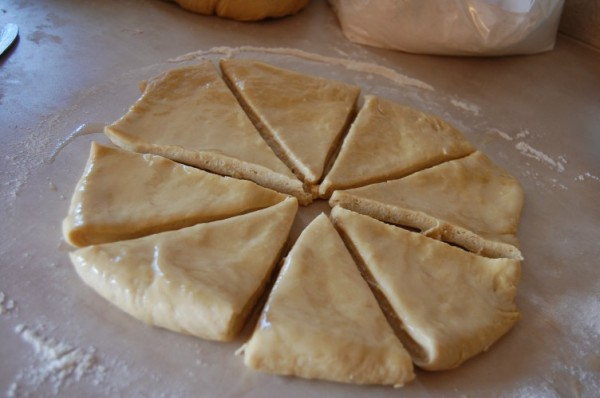
\includegraphics[width=200px]{images/divide.jpg}\end{center}
  \begin{center}\textbf{git submodule }add $<$repository-url$>$\end{center}
\end{frame}